%!TEX program = xelatex
\documentclass{beamer}

%\usepackage{ctex}
\usepackage{xeCJK}
\usepackage{algorithm}
\usepackage{algorithmic}
\usepackage{graphicx}
\usepackage{fourier}
\beamertemplatetransparentcovereddynamicmedium

\usepackage{listings}
\usepackage{color}

\usetheme{Darmstadt}
\usecolortheme{whale}

\definecolor{mygreen}{rgb}{0,0.6,0}
\definecolor{mygray}{rgb}{0.5,0.5,0.5}
\definecolor{mymauve}{rgb}{0.58,0,0.82}
\setbeamertemplate{footline}[frame number]

\lstset{
  backgroundcolor=\color{white},   % choose the background color; you must add \usepackage{color} or \usepackage{xcolor}
  basicstyle=\footnotesize,        % the size of the fonts that are used for the code
  breakatwhitespace=false,         % sets if automatic breaks should only happen at whitespace
  breaklines=true,                 % sets automatic line breaking
  captionpos=b,                    % sets the caption-position to bottom
  commentstyle=\color{mygreen},    % comment style
  escapeinside={\%*}{*)},          % if you want to add LaTeX within your code
  extendedchars=true,              % lets you use non-ASCII characters; for 8-bits encodings only, does not work with UTF-8
  frame=single,                    % adds a frame around the code
  keepspaces=true,                 % keeps spaces in text, useful for keeping indentation of code (possibly needs columns=flexible)
  keywordstyle=\bfseries\color{blue},% keyword style
  language=Java,                    % the language of the code
  morekeywords={constexpr,decltype},% if you want to add more keywords to the set
  numbers=left,                    % where to put the line-numbers; possible values are (none, left, right)
  numbersep=5pt,                   % how far the line-numbers are from the code
  numberstyle=\tiny\color{mygray}, % the style that is used for the line-numbers
  rulecolor=\color{black},         % if not set, the frame-color may be changed on line-breaks within not-black text (e.g. comments (green here))
  showspaces=false,                % show spaces everywhere adding particular underscores; it overrides 'showstringspaces'
  showstringspaces=false,          % underline spaces within strings only
  showtabs=false,                  % show tabs within strings adding particular underscores
  stepnumber=1,                    % the step between two line-numbers. If it's 1, each line will be numbered
  stringstyle=\color{mymauve},     % string literal style
  tabsize=4,                       % sets default tabsize to 2 spaces
  %title=\lstname                  % show the filename of files included with \lstinputlisting; also try caption instead of title
  %caption=\lstname
}

\begin{document}
	\begin{frame}[containsverbatim]
		\title{Master}
		\subtitle{Compiler 2016}
		\author{Zihao Ye\\ACM Class 2014}
		\date{\today}
		\titlepage
	\end{frame}

	\begin{frame}
		\begin{block}{About name}
		Master Compiler was named after a role in Doctor Who: The Master.
		\end{block}
		\begin{block}{Properties}
		It's a simple(slow) \& naive(not efficient) implementation of a superset of Mx* in which member function/method is permitted.
		\end{block}
	\end{frame}
	\section{Structure} % (fold)
	\label{sec:structure}
	
	% section structure (end)
	\begin{frame}
		\frametitle{Structure}
		\begin{block}{Procedures}
		\begin{itemize}
			\item
			Parser: From source code to AST.
			\item
			From AST to Linear IR.
			\item
			From Linear to CFG(with a subtle optimization).
			\item
			Register allocation.
			\item
			From IR to MIPS.
		\end{itemize}
		\end{block}
	\end{frame}

	\section{Front End} % (fold)
	\label{sec:front_end}
	
	% section front_end (end)
	\begin{frame}
		\frametitle{Front End}
		\begin{block}{Parser}
		ANTLR: source code -> CST.
		\end{block}
		\pause
		\begin{block}{AST}
		Convert CST to AST:
			\begin{description}
				\item[Firstlistener:]
				
				Initialize, and collect all class names.
				\item[Secondlistener:]
				
				Collect all function names and arguments.
				\item[Thirdlistener:]
				
				Construct the whole AST.
			\end{description}
		\end{block}
	\end{frame}

	\begin{frame}
		\frametitle{Front End}
		\begin{block}{Structure of AST}
		\centering
		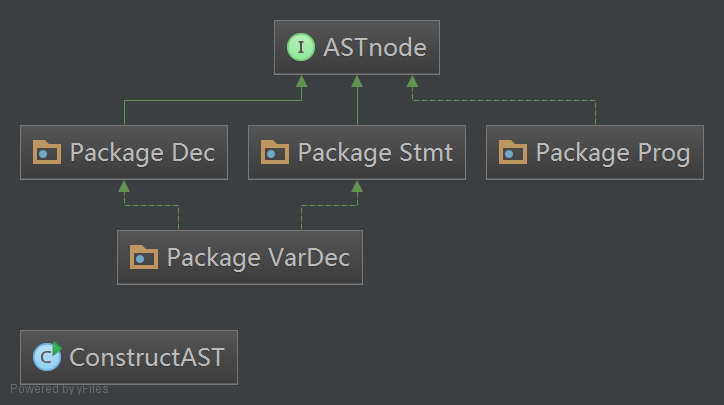
\includegraphics[height = 1in]{AST.png}
		\end{block}
	\end{frame}

	\begin{frame}
		\frametitle{Front End}
		\begin{block}{Some special AST nodes:}
		\begin{description}
			\item[Type:] 
			ClassDec is used to distinguish different types.(Builtin classs such as int, bool, string are defined in the Utility.h)
			\item[Symbol:]
			VarDec is used to distinguish different symbols.
		\end{description}
		\end{block}
	\end{frame}

	\begin{frame}
		\frametitle{Front End}
		\begin{block}{Structure of Symbol Table}
			Symbol table(called Scope) is nested in AST nodes. 
			\centering
			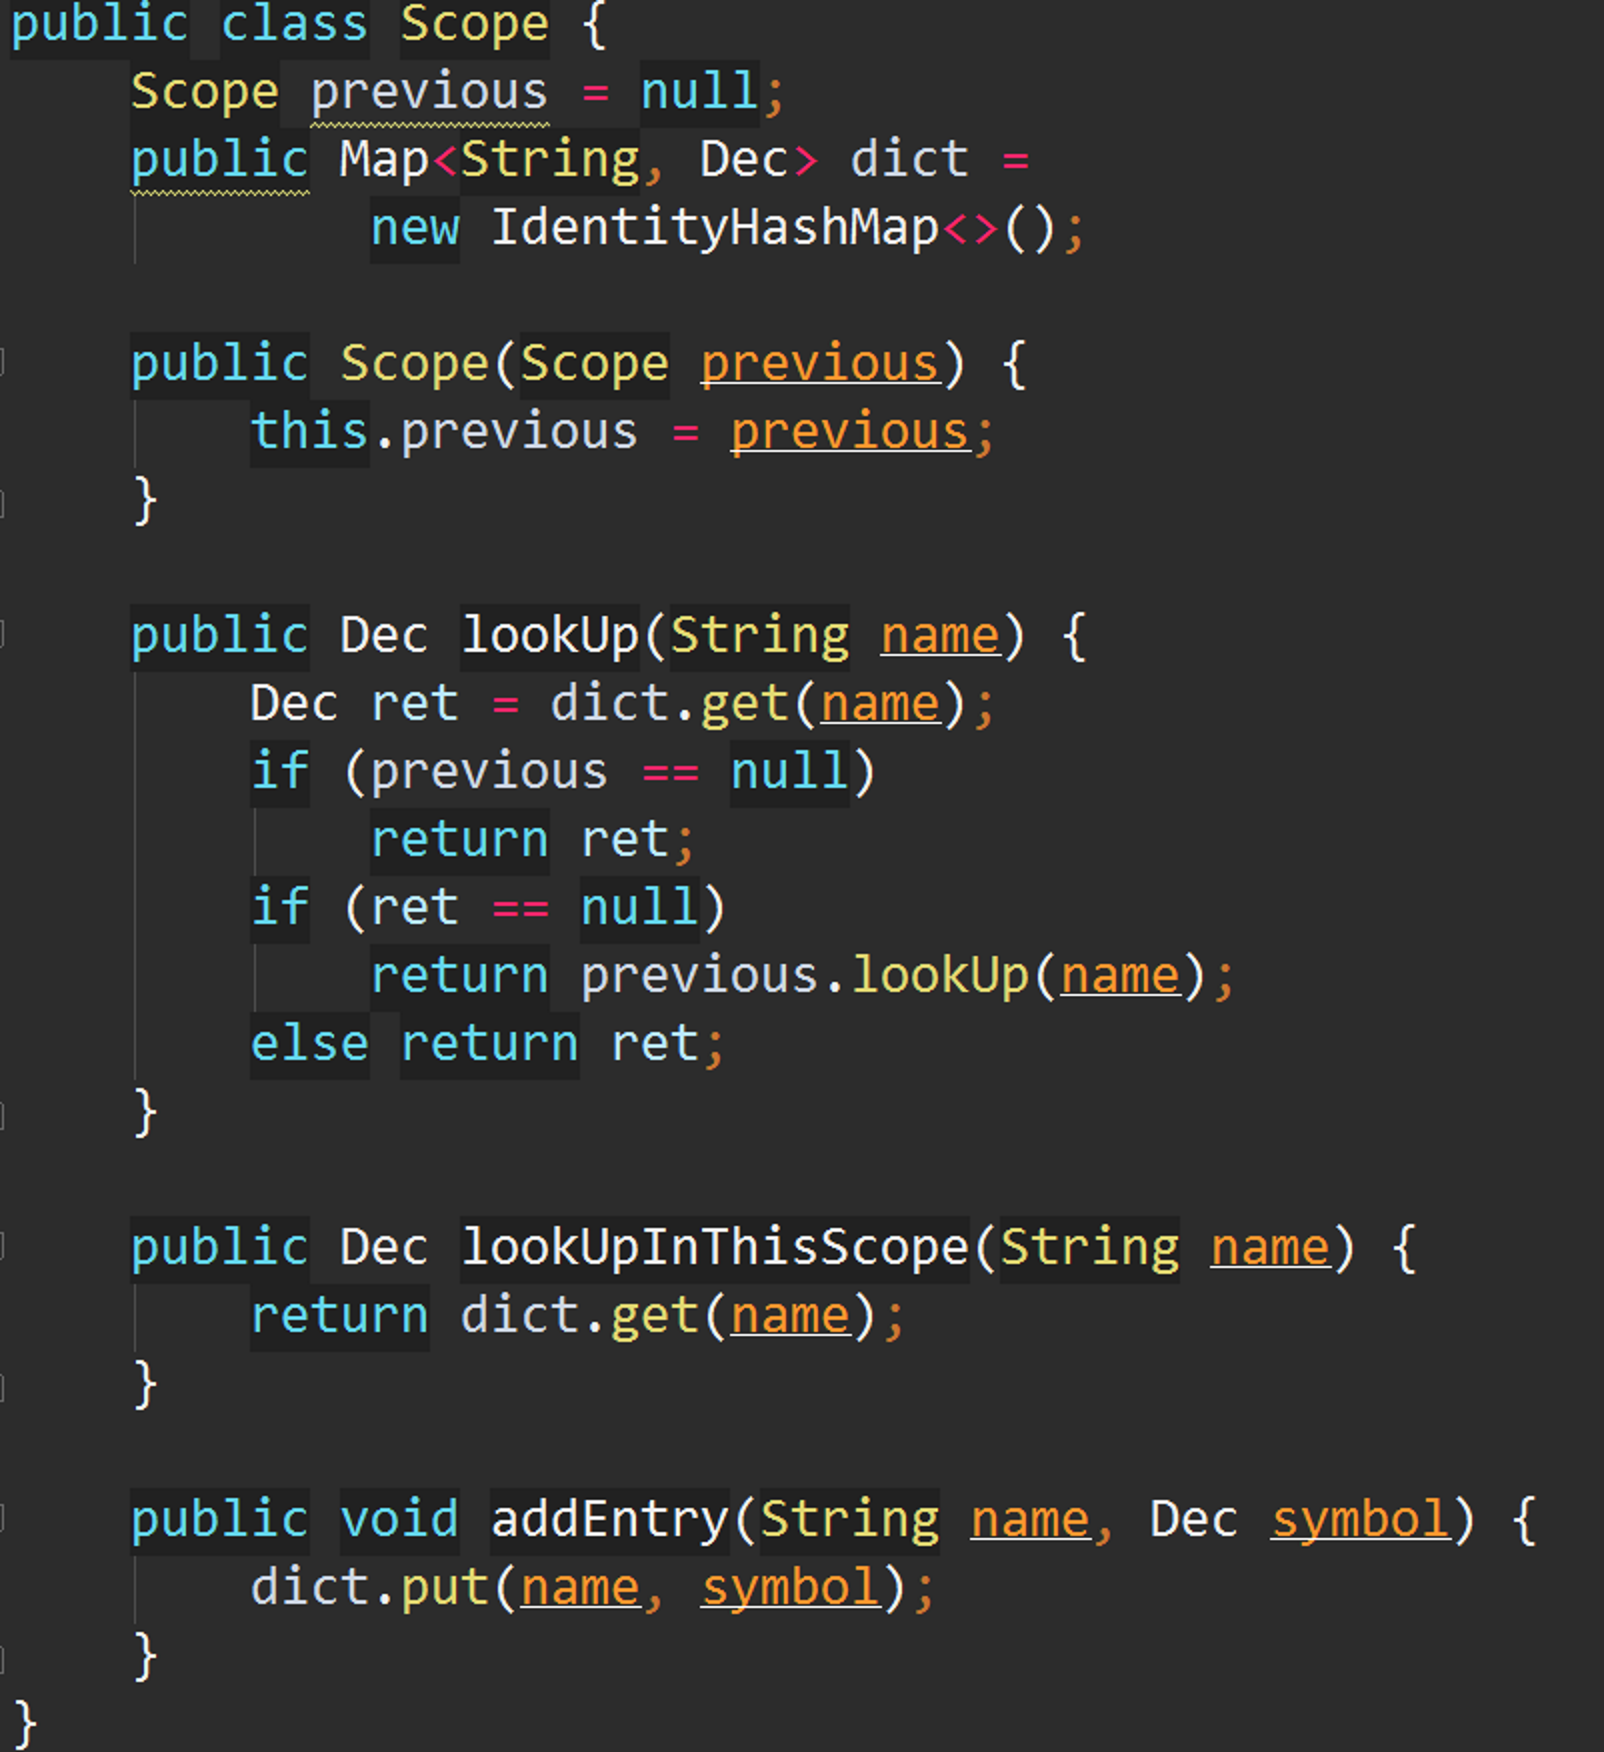
\includegraphics[height = 2in]{scope.png}
		\end{block}
	\end{frame}

	\section{Back End} % (fold)
	\label{sec:back_end}
	
	% section back_end (end)
	\begin{frame}
		\frametitle{Back End}
		\begin{block}{Linear IR \& CFG}
		\begin{itemize}
			\item
			IR design: a three-address IR with infinite virtual registers(LLIR).
			\item 
			Generate linear IR: Prog.emit();
			\item
			Convert linear IR to CFG: divide linear IR into basicblocks and collect all basicblocks in the same function together.
		\end{itemize}
		\end{block}
	\end{frame}

	\begin{frame}
		\frametitle{Back End}
		\begin{block}{A trivial optimizations}
		\begin{itemize}
			\item
			Since there are some basicblocks like:
			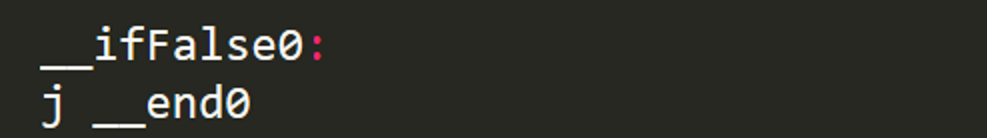
\includegraphics[height=0.5in]{label.png}

			combining these labels become necessary. By using the same method as union-find set, we can replace each label with the nearest one that really make sense.
		\end{itemize}
		\end{block}
	\end{frame}

	\begin{frame}
		\begin{block}{Liveness Analysis \& Register Allocation}
		\begin{description}
			\item[Interference graph]: 
			
			Iteration algorithm, instruction by instruction.
			\item[Coloring]: 
			
			Greedy algorithm(color the vertex with minimum degree each step).
		\end{description}
		\end{block}
	\end{frame}

	\begin{frame}
		\begin{block}{Liveness Analysis \& Register Allocation}
		\begin{itemize}
			\item \$v0, \$v1 are used to store temporary variables of Three-address code.
			\item \$a0, \$a1, \$a2 are used as first 3 function arguments.
			\item Most of other machine registers(\$ra, \$at, \$0, exclusively)ar used in register allocation.
			\item MIPS instructions like `move \$r0, \$r0' will be eliminated.
		\end{itemize}
		\end{block}
	\end{frame}

	\section{Example} % (fold)
	\label{sec:example}
	
	% section example (end)
	\begin{frame}
		\begin{block}{Example}
		Member function:

		\centering
		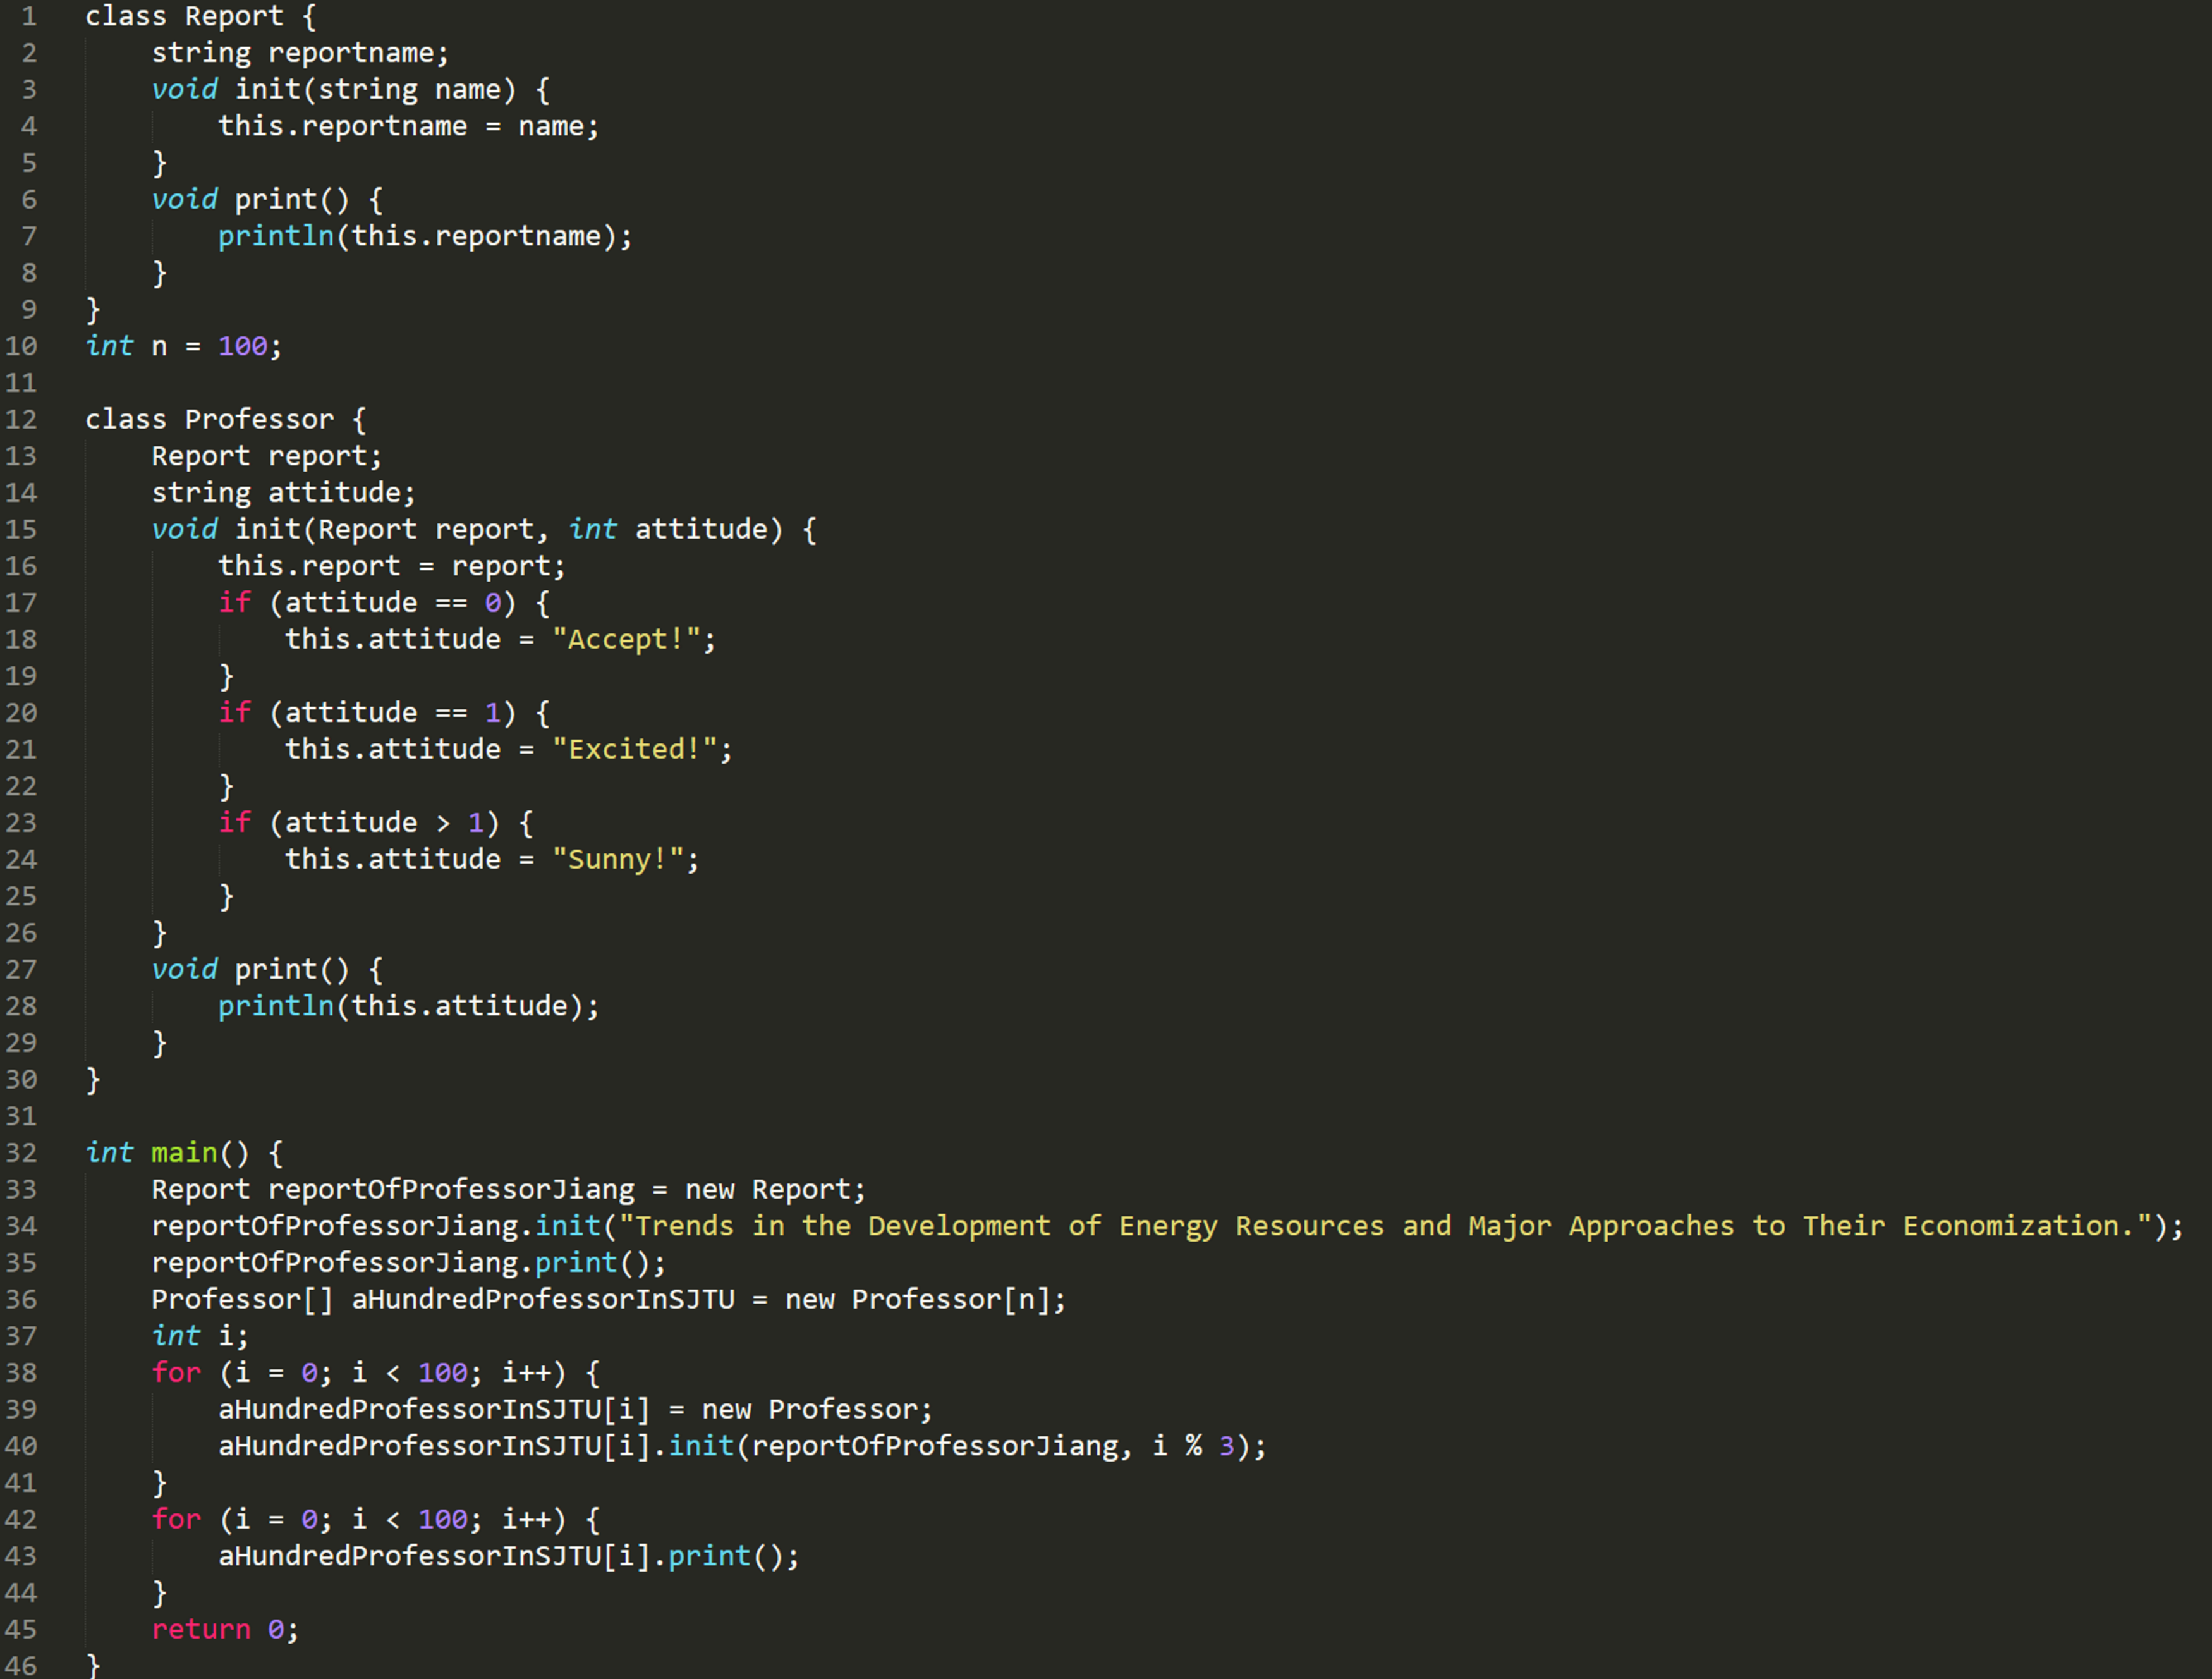
\includegraphics[height=2in]{applyForProfessor.png}
		\end{block}
	\end{frame}

	\begin{frame}
		\begin{block}{Example}
		Member function:

		\centering
		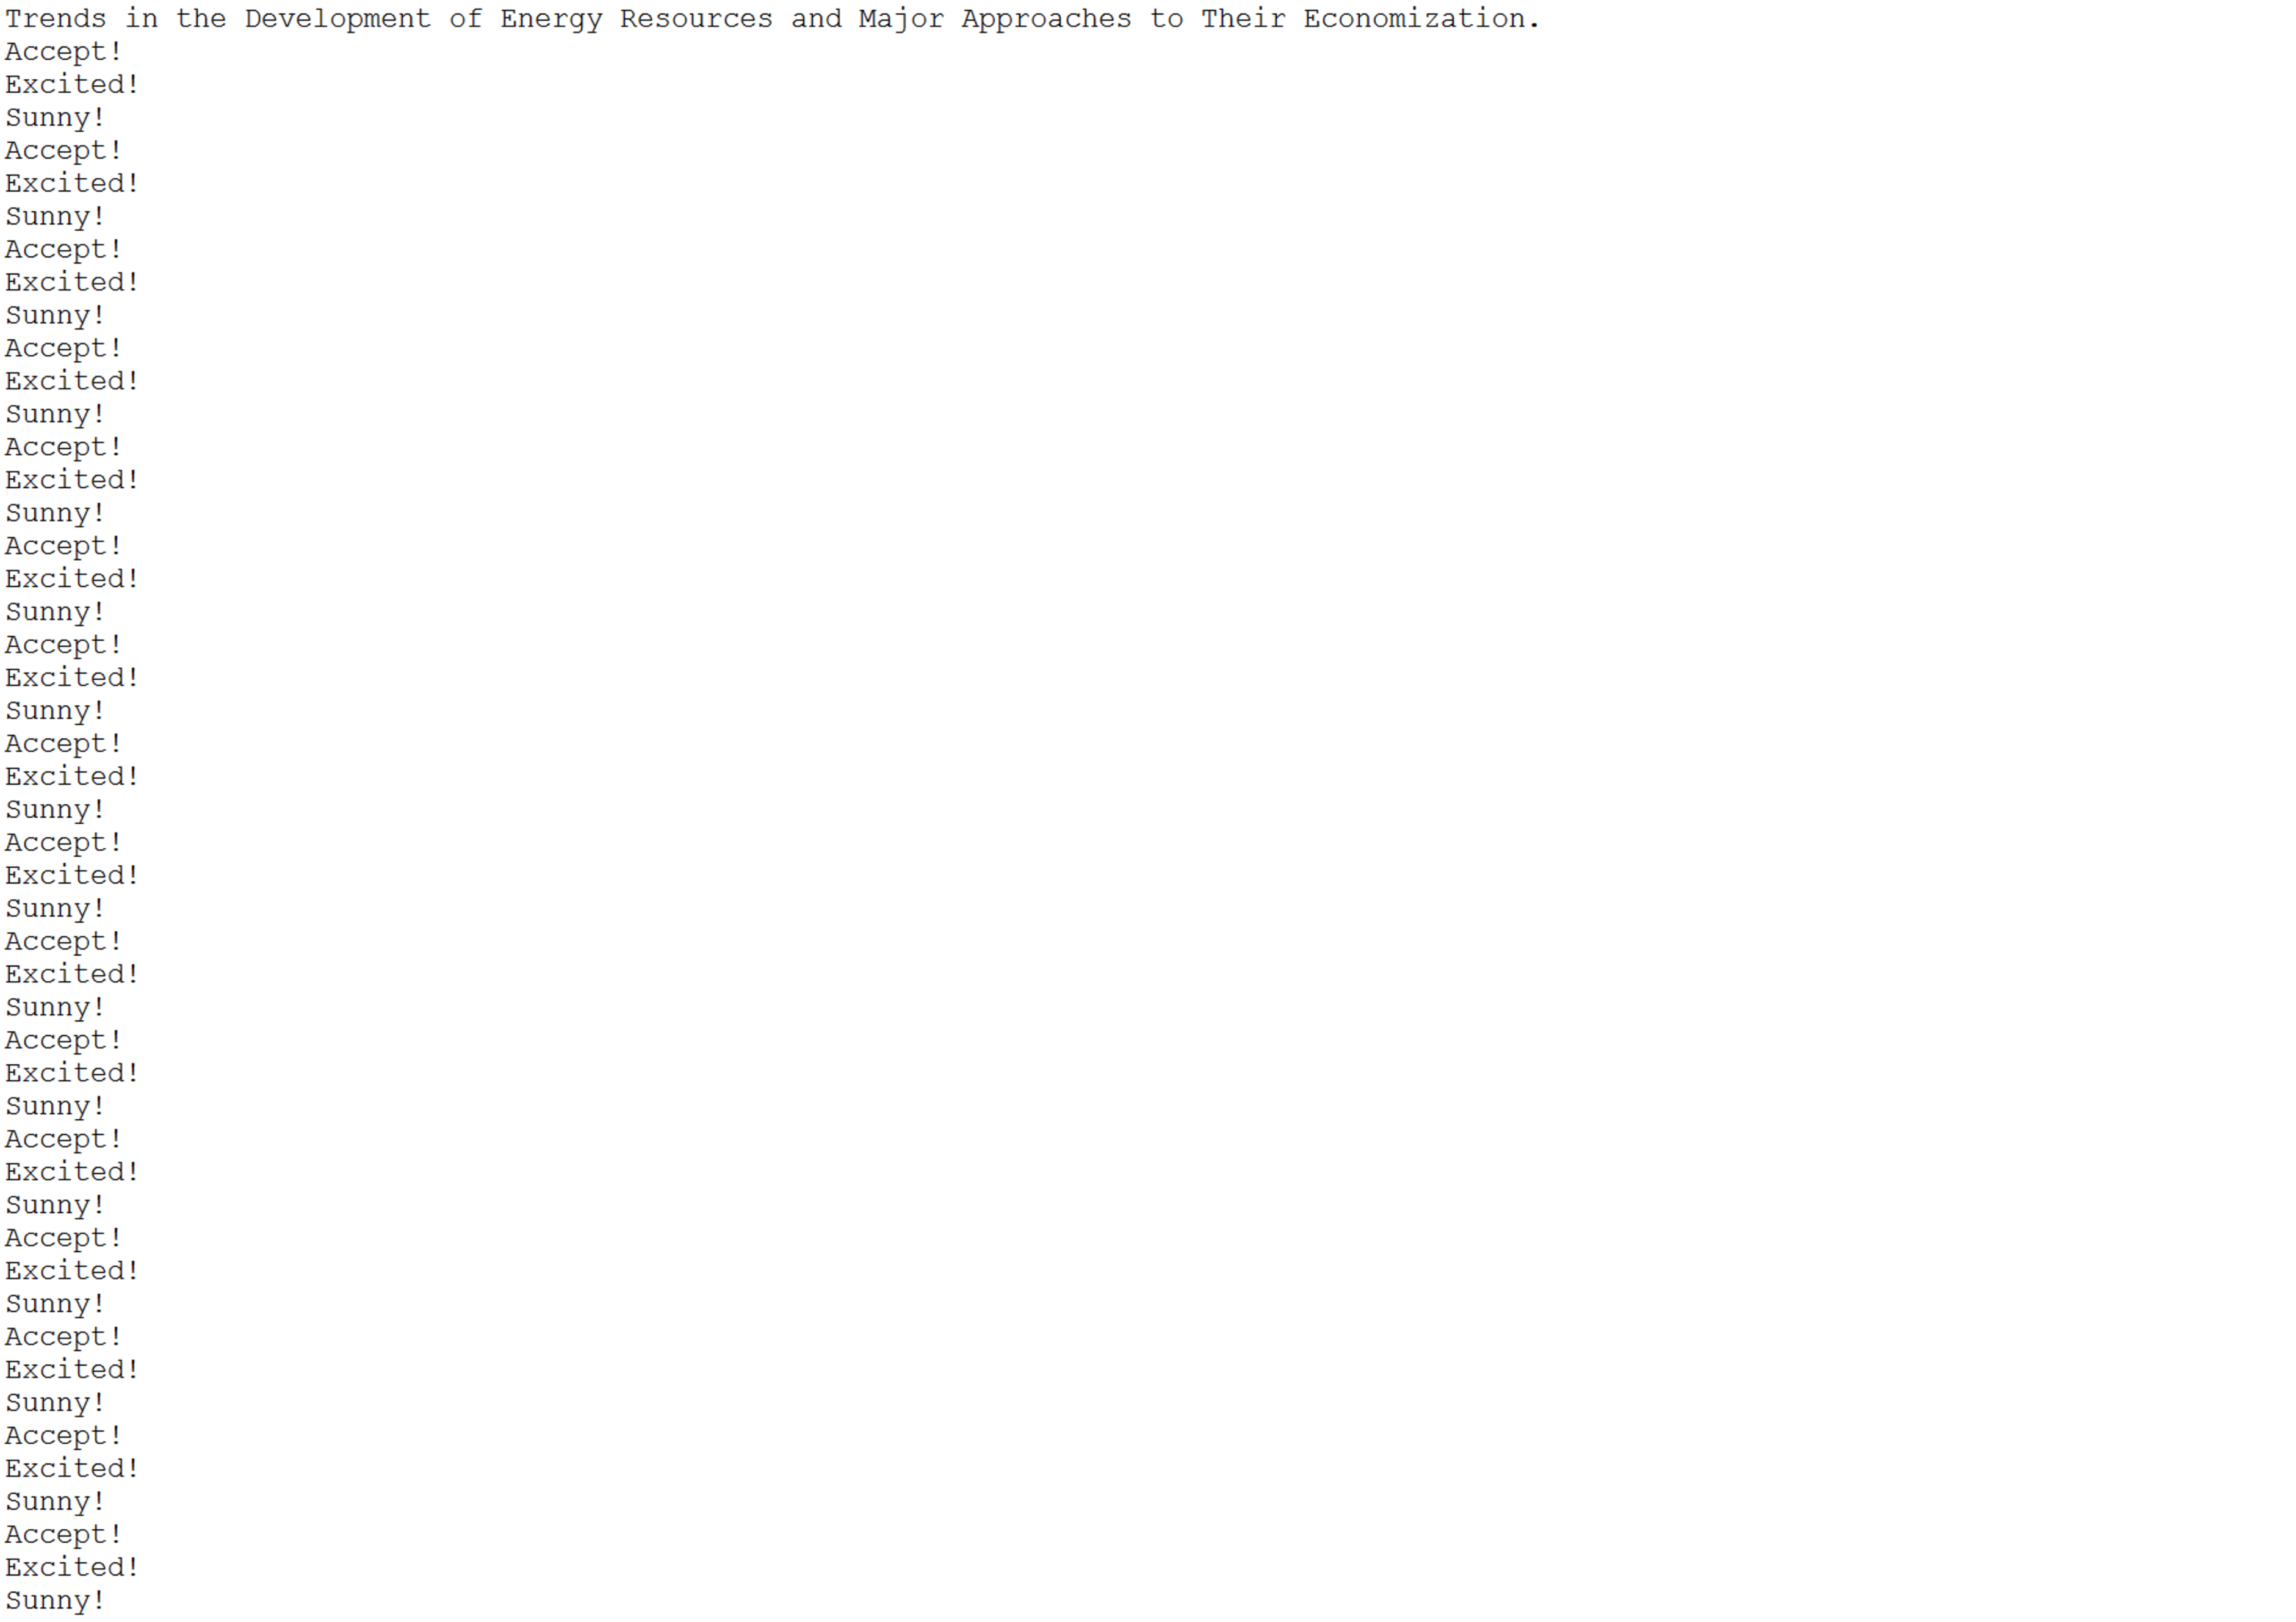
\includegraphics[height=2in]{professor.png}
		\end{block}
	\end{frame}
	
	\section{Thanks} % (fold)
	\label{sec:thanks}
	
	% section thanks (end)
	\begin{frame}
		\begin{block}{Thanks}
			\begin{itemize}
				\item 
				I would like to thank all of our TAs for their hard work.

				\item
				I would like to thank Lequn Chen for his generous help \& programs for unit test.

				\item
				I would like to thank Zhijian Liu for some of his suggestions.

				\item
				I would like to thank Tianyao Chen and Yurong You for their builtin functions.
			
			\end{itemize}
			\centering
			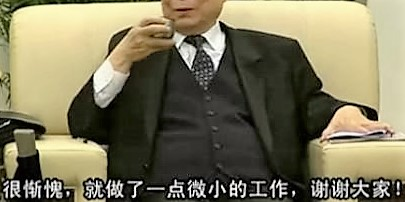
\includegraphics[height=1in]{cankui.jpg}
		\end{block}
	\end{frame}
\end{document}